\documentclass[a4paper]{article}

\usepackage[english]{babel}
\usepackage[utf8]{inputenc}
\usepackage{amsmath}
\usepackage{graphicx}
\usepackage[colorinlistoftodos]{todonotes}

\title{Advanced Summary of the "Deep Learning" book by Goodfellow, Bengio and Courville}

\author{Jérémy Scheurer}

\date{\today}

\begin{document}
\maketitle

\begin{abstract}
This is my personal summary of the book "Deep Learning" by Bengion, Goodfellow and Courville. I cover the chapters relevant to deep learning, i.e. 6-9. Note that before reading this book I already had a good understanding of Neural Networks, so I did not make notes of the more simple concepts and ideas. Also I will refrain from citing each individual passage that I literally copy from the book as this summary is intended for personal use. 
\end{abstract}

\section{6: Feedforward Networks}
\label{sec:feedforward}
\subsection{Introduction}
\begin{itemize}
\item We try to learn the parameters $\theta$ of a function $y=f(x,\theta)$
\item Each layer has many units acting in parallel. Each unit(neuron) is vector to scale and thus from layer to layer we have a vector to vector relationship.
\item Classical example of why we need a non-linear function: 
\begin{center}
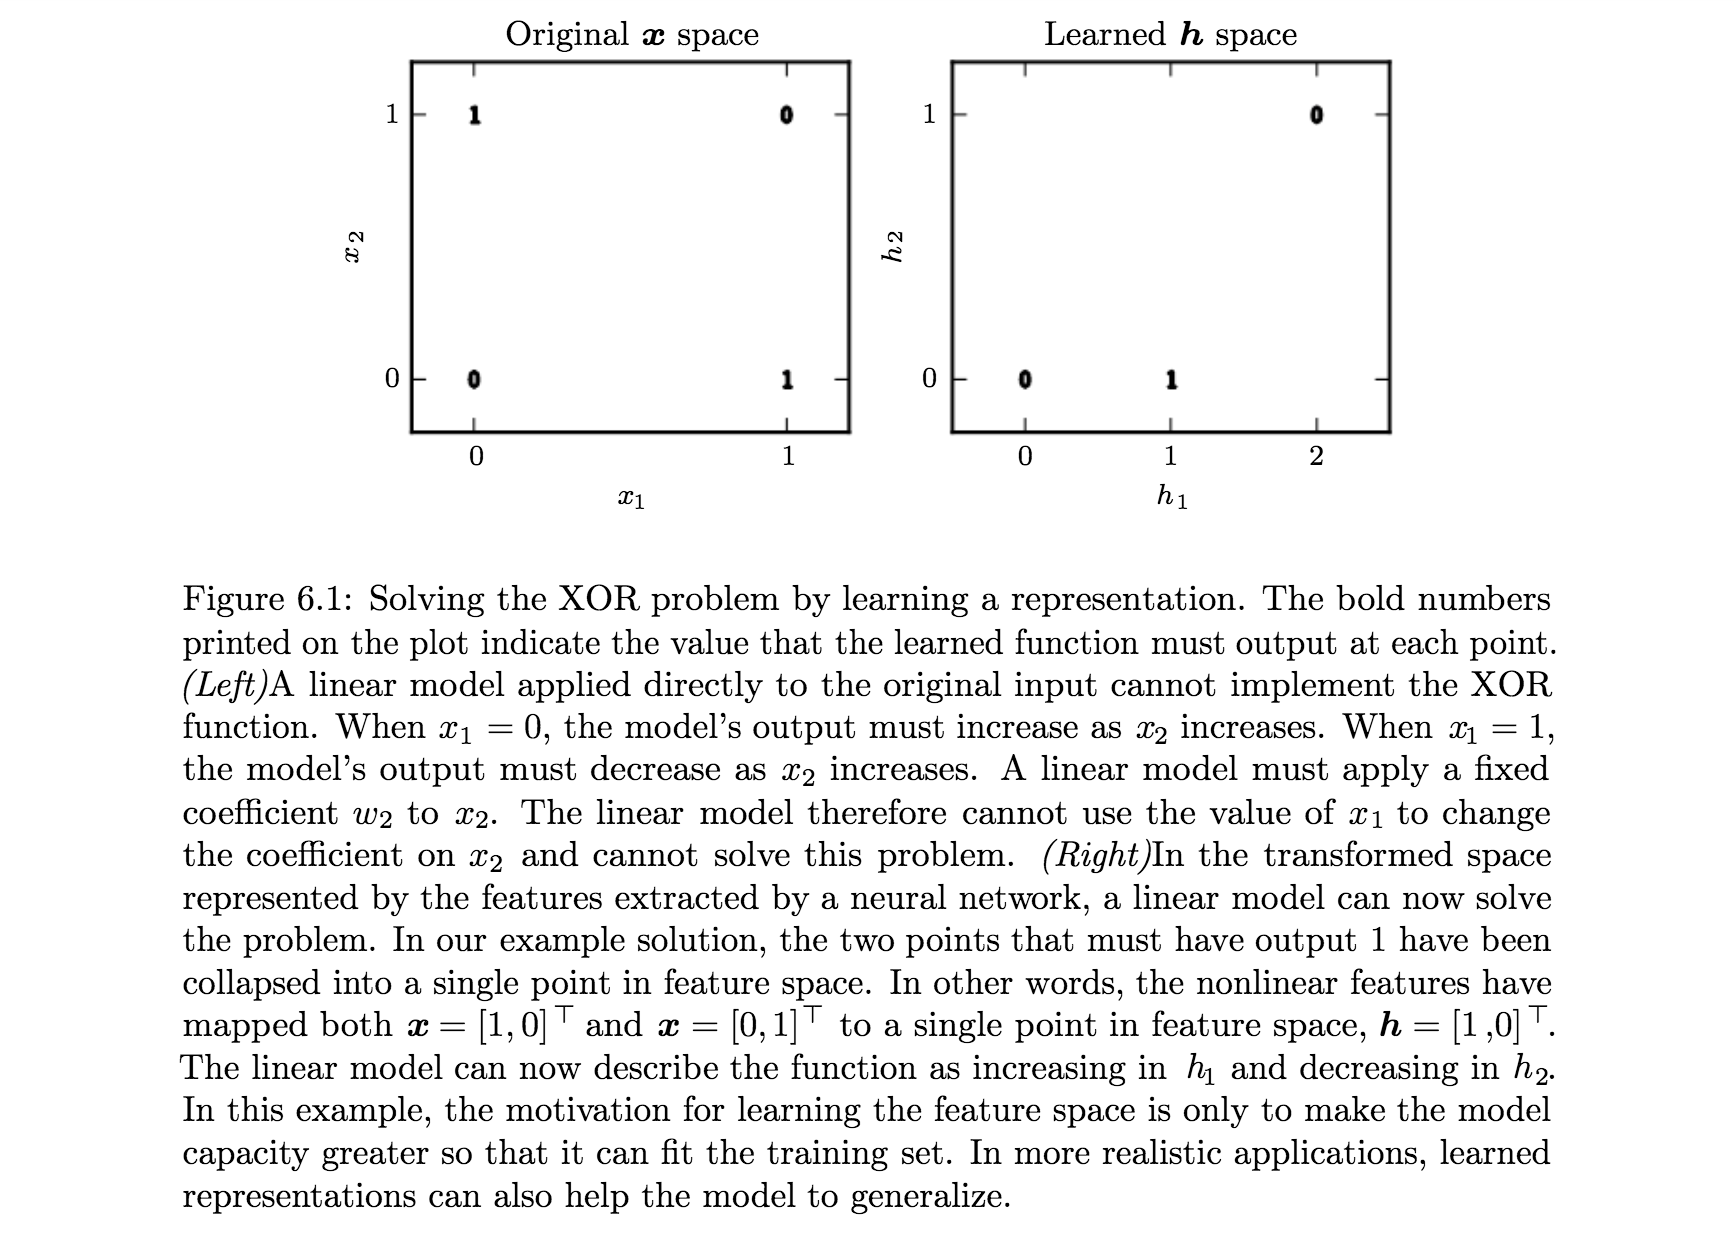
\includegraphics[width = \textwidth, height=7cm]{image/xor.png}
\end{center}


\item We need non-linear functions $\phi$. How to choose such a function: 
	\begin{itemize}
	\item One option is to use a very generic $\phi$, such as the infinite-dimensional $\phi$ that is implicitly used by kernel machines based on the RBF kernel. If $\phi(x)$ is of high enough dimension, we can always have enough capacity to fit the training set, but generalization to the test set often remains poor. Very generic feature mappings are usually based only on the principle of local smoothness and do not encode enough prior information to solve advanced problems. 
    \item Another idea is to manually engineer the function as was usually done with kernels for specific tasks. This is very hard and does not generalize to other tasks. 
    \item The correct approach we follow in deep learning is  to get a generic function and let the network find the parameters which maximize this function. We have $$y = f(x,\theta,w) = \phi(x,\theta)^T w$$ The parameters $\theta$ are here to learn $\phi$ from a broad class of functions and w is here to map it to the output. In this approach we sacrifice the convexity but gain other things. First of all it is still very general such as in the first approach and second of all we get very specific functions such as in the second approach. 
	\end{itemize}
\item One applies the non-linear function usually element wise to the units. The standard function is the Rectified Linear unit. 
\begin{center}
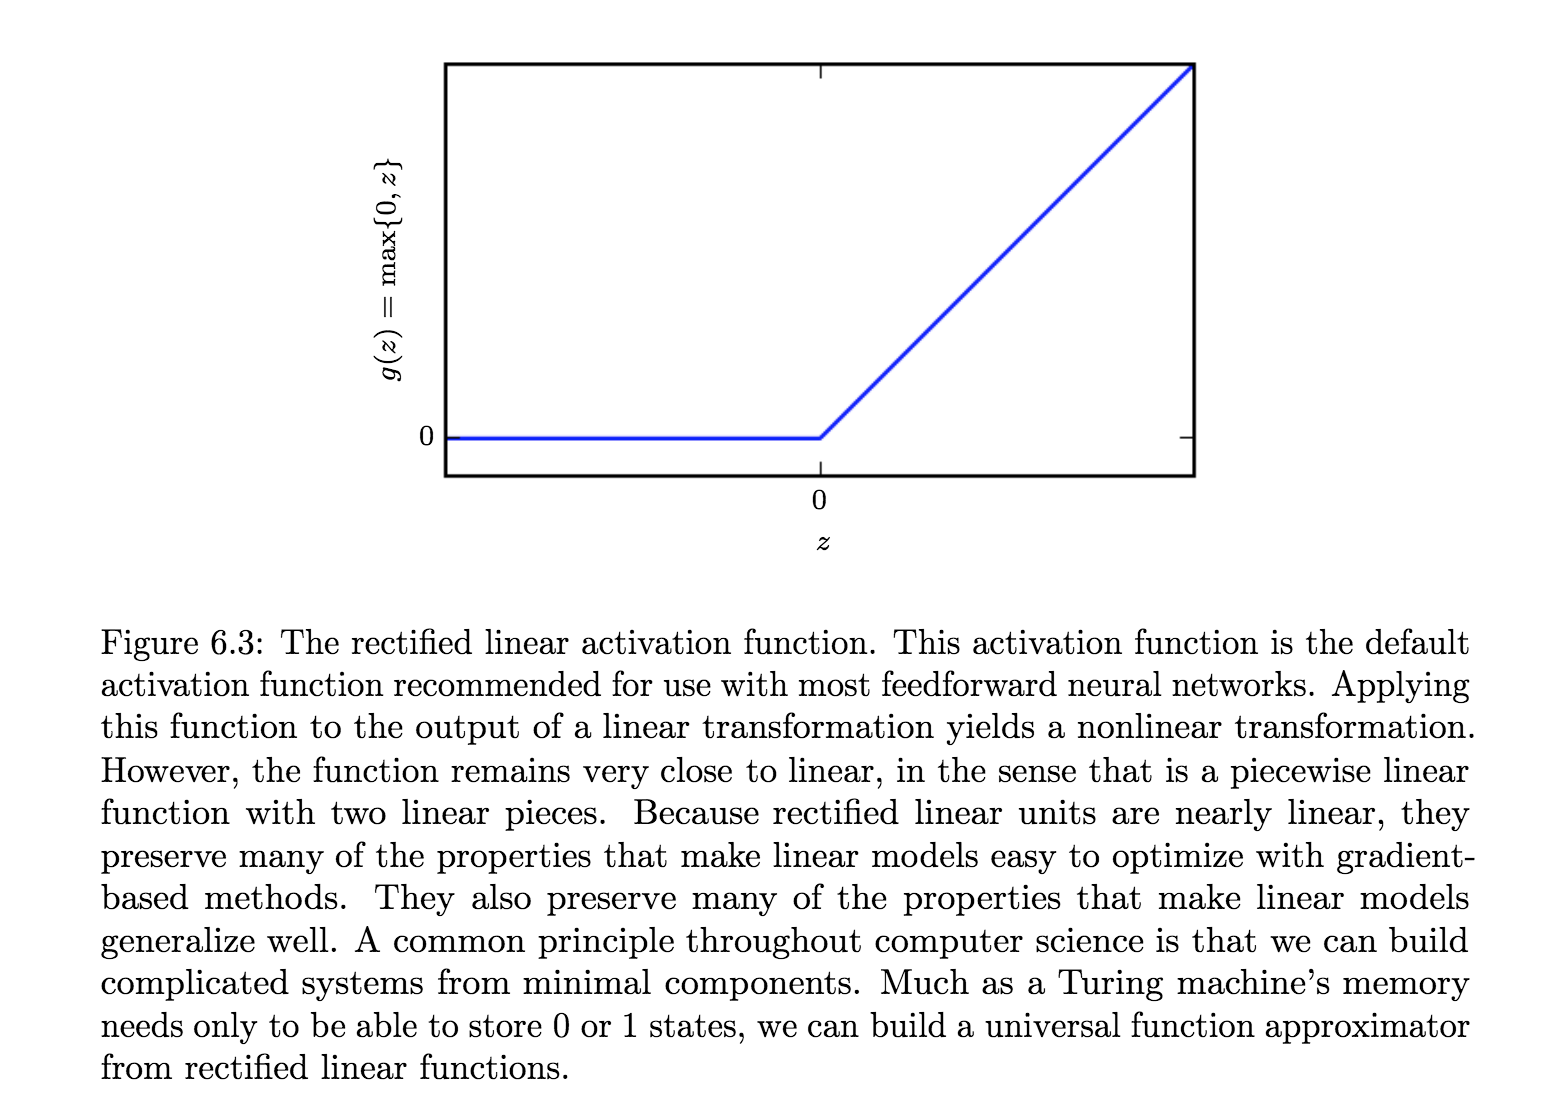
\includegraphics[width=\textwidth]{image/relu.png}
\end{center}
\end{itemize}

\subsection{Gradient Based Learning}
\begin{itemize}
\item Machine learning models are build by defining and optimization technique, a cost function and a model family. The difference is that now we have non-linearity thus it is not a convex optimization problem anymore. Note that it is much more sensitive to initial values. So initialize the weights to small random variables and the biases to zero.
\item Most modern neural networks are trained using maximum likelihood. This means that the cost function is simply the negative log-likelihood,equivalently describe by: 
$$J(\theta) = -E_{x,y~p_{data}} log(p_{model}(y|x)$$
the advantage of this cost function is that it relieves us of the work of designing a cost function for every application
\item The gradient should be large and predictable to serve as good guide for the learning task. Functions that saturate (become very flat) undermine this objective because they make the gradient become very small. In many cases this happens because the activation functions used to produce the output of the hidden units or the output units saturate. The negative log-likelihood helps to avoid this problem for many models. Several output units involve an exp function that can saturate when its argument is very negative. The log function in the negative log-likelihood cost function undoes the exp of some output units.
\item Using variational calculus one can also defined a cost function which tries to find a function which satisfies a certain property. Here an example: 
$$ f* = argmin_f E_{x,y~p_{data}}||y-f(x)||^2$$ which then yields 
$$f*(x) = E_{y~p_{data(y|x)}}[y]$$
So in other words, if we could train on infinitely many data samples from the true data generating distribution, we could get a function which predicts the mean of y given x. 
\item An important factor is also how to produce the outputs from the last layer. One can use just linear units(dense network with no activation function) to produce the output. This works great with gradient descent. On the other hand when one does binary classification, one needs something different. One way would be to do the same as above but frame it in the following way: 
$$P(y=1|x) = max(0, min(1, w^th+b))$$
But as soon as the result strays out of the interval [0,1] the gradient becomes 0 which is bad. To keep a "good" gradient one uses a sigmoid function combined with maximum likelihood. We can reformulate it in terms of a probability distribution which leaves and exp in there. As mentioned before this can saturate. But because we take the log of th probability, the exp is gone again. 
For multi-label classification, one uses a softmax. Note that this can sometimes also be used inside a neural net as a hidden unit. This is done if one wants to select between n options. Using the log likelihood with a softmax works well, but using a MSE with a softmax does not.  
\end{itemize}

\subsection{Hidden Units}
\begin{itemize}
\item Most hidden units take an input x and apply an affine transformation to it $z = w^tx+b$ and then apply some sort of non-linear function to it. 
\item Basic non-linear function one is RELU (max(0,z) but there are many others. RELU is easy to train, because it is nearly linear.  Note that it is not differentiable at 0, but one does oftentimes not care about it, because usually the training loss never reaches 0 but comes close to it. One usually sets b to some small positive value(ex. 0.1), because this usually allows the gradient to pass(because the relu is active) for most initial inputs. 
A drawback of RELU's is that they cannot learn from examples for which their activation is 0. There are variants which try to address this problem. 
\item If a hidden unit is not differentiable at a specific point it can often also be, because its  left and right differential are not equal to each other which they should be. But because of numerical instability of working on a finite precision machine, it is very unlikely that this exact value is ever reached. More often a  value with a small epsilon around the non-differential value is reached. So in practice implementations usually just give the left or the right differential. 

\item Logistic Sigmoid = $\sigma(z)$ and hyperbolic tangent = $tanh(z) = 2\sigma(z) -1$. Unfortunately sigmoids saturate over most of their range, except around 0. The reason they are accepted as output functions is that certain cost functions remove their bad properties. The tanh function usually works better and resembles the identity function more closely. 
\end{itemize}

\subsection{Architecture Design}
\begin{itemize}
\item Deeper layers usually need fewer parameters i.e. units per layer and generalize better. On the other hand they are harder to train. 
\item The universal approximation theorem says that even an NN with one hidden layer could approximate any function, assuming it has enough hidden units. So we know, any function can be represented by a NN, but we do not know if the training algorithm is able to learn it. First because it might not be able to learn the correct parameters and second because it might overfit and thus learn the wrong function.
\item Montufar et al. showed that functions representable with a deep rectifier net can require an exponential number of hidden units with a shallow (one hidden layer) network. More precisely, they showed that piecewise linear networks (which can be obtained from rectifier nonlinearities or maxout units) can represent functions with a number of regions that is exponential in the depth of the network. Figure 6.5 illustrates how a network with absolute value rectification creates mirror images of the function computed on top of some hidden unit, with respect to the input of that hidden unit. Each hidden unit specifies where to fold the input space in order to create mirror responses (on both sides of the absolute value nonlinearity). By composing these folding operations, we obtain an exponentially large number of piecewise linear regions that can capture all kinds of regular (e.g., repeating) patterns.
\begin{center}
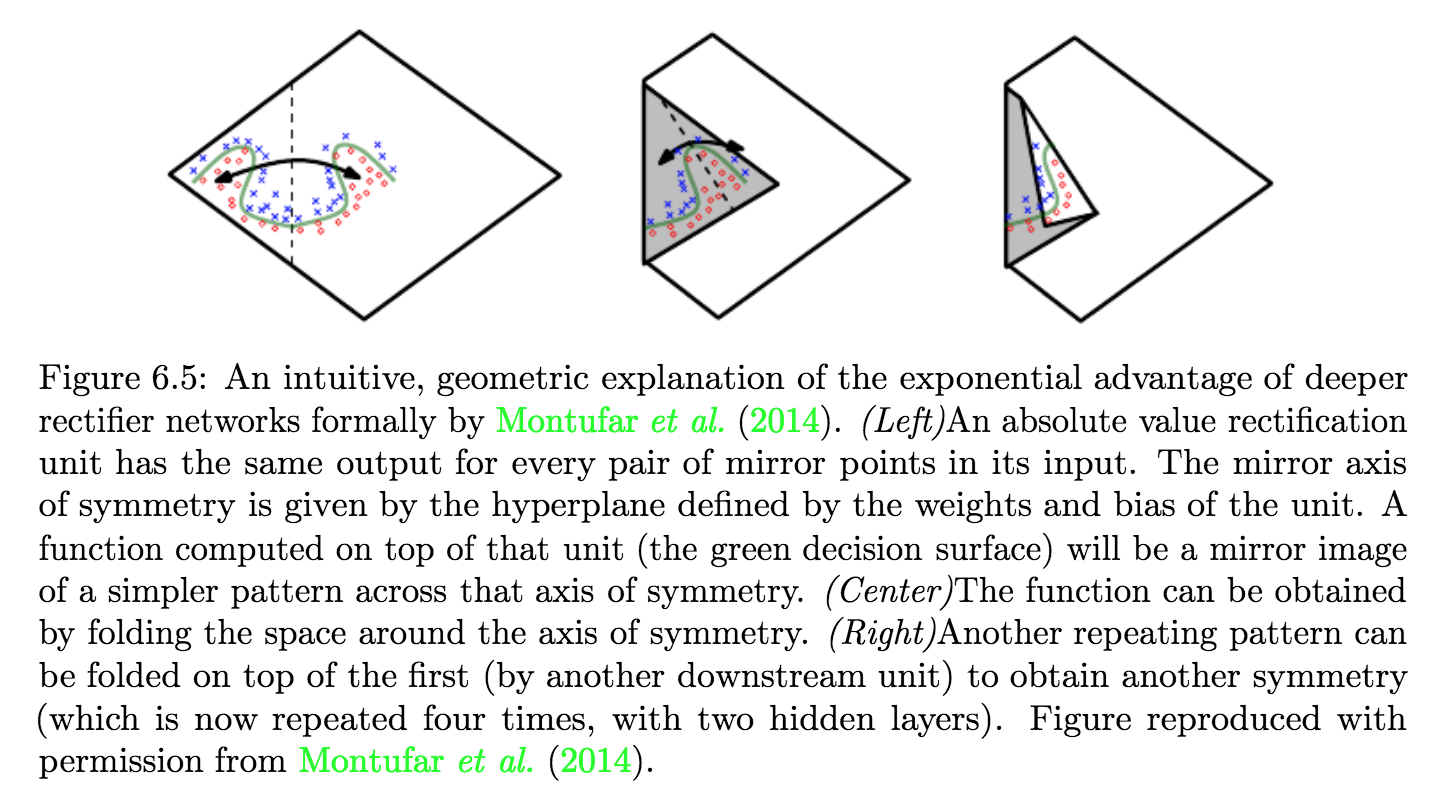
\includegraphics[width=\textwidth]{image/folding.png}
\end{center}

\item Some architectures use skip connections, i.e. direct connections from one unit to another one ex. 2 layers ahead. This allows for the gradient to flow better. Also one unit can have connections to all other units of the next layer or also only to one ore multiple units of the next layer. This yields fewer parameters, which might improve the results and is quicker to train. 
\end{itemize}

\subsection{Backpropagation and other Differential Algorithms}
\begin{itemize}
\item An important differentiation has to be made with respect to backprop. This is only the algorithm which tells us how a gradient flows through the network. The actual calculation of the gradient can be done with SGD, Adam, Pegasos etc. 
\item Usually one computes the gradient of the Cost-function with respect to its parameters. 
\item The Basic idea is just to apply the chain rule of differential calculus. It is kind of tedious to note down, so I refer to the book. Also there is more on how Deep Learning Software do backprop.
\end{itemize}


\begin{thebibliography}{9}
\bibitem{nano3}
  K. Grove-Rasmussen og Jesper Nygård,
  \emph{Kvantefænomener i Nanosystemer}.
  Niels Bohr Institute \& Nano-Science Center, Københavns Universitet

\end{thebibliography}
\end{document}